\section{Sequential Attend-Infer-Repeat}
\label{sec:sqair}

\begin{figure}
    \centering
    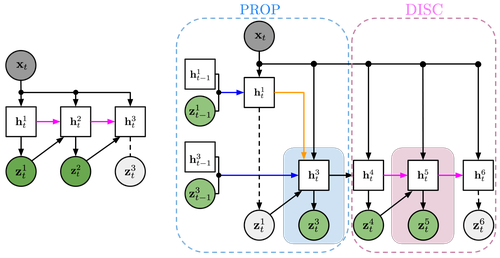
\includegraphics[width=.7\linewidth]{figures/SQAIR/air_sqair_inference}
    \caption{
    \textit{Left}: 
        Inference in \gls{AIR}. 
        The \textcolor{pink}{pink \gls{RNN}} attends to the image sequentially and produces one latent variable $\bzt^i$ at a time. 
        Here, it decides that two latent variables are enough to explain the image and $\bzt^3$ is not generated.
    % 
    \textit{Right}:
        Inference in \gls{SQAIR} starts with the \gls{prop} phase.
        \gls{prop} iterates over latent variables from the previous time-step $t-1$ and updates them based on the new observation $\bxt$.
        The \textcolor{blue}{blue \gls{RNN}} runs forward in time to update the hidden state of each object, to model its change in appearance and location throughout time. 
        The \textcolor{orange}{orange \gls{RNN}} runs across all current objects and models the relations between different objects.
        Here, when attending to $\bz^1_{t-1}$, it decides that the corresponding object has disappeared from the frame and \textit{forgets} it.
        Next, the \gls{disc} phase detects new objects as in \gls{AIR}, but in \gls{SQAIR} it is also conditioned on the results of \gls{prop}, to prevent rediscovering objects. See \Cref{fig:sqair_inf_detail} for details of the colored \glspl{RNN}.}
    \label{fig:sqair_inf_flow}
\end{figure}


While capable of decomposing a scene into objects, \gls{AIR} only describes single images. Should we want a similar decomposition of an image sequence, it would be desirable to do so in a temporally consistent manner. For example, we might want to detect objects of the scene as well as infer dynamics and track identities of any persistent objects.
Thus, we introduce  \glsreset{SQAIR} \gls{SQAIR}, whereby \gls{AIR} is augmented with a \gls{SSM} to achieve temporal consistency in the generated images of the sequence.
The resulting probabilistic model is composed of two parts:  \glsreset{disc}\gls{disc}, which is responsible for detecting  (or introducing, in the case of the generation) new objects at every time-step (essentially equivalent to \gls{AIR}), and \glsreset{prop}\gls{prop}, responsible for updating (or forgetting) latent variables from the previous time-step given the new observation (image), effectively implementing the temporal \gls{SSM}.
We now formally introduce \gls{SQAIR} by first describing its generative model and then the inference network.

\textbf{Generative Model}
The model assumes that at every-time step, objects are first propagated from the previous time-step (\gls{prop}). Then, new objects are introduced (\gls{disc}). 
Let $t \in \mathbb{N}$ be the current time-step.
Let $\mathcal{P}_t$ be the set of objects propagated from the previous time-step and let $\mathcal{D}_t$ be the set of objects discovered at the current time-step, and let $\mathcal{O}_t = \mathcal{P}_t \cup \mathcal{D}_t$ be the set of all objects present at time-step~$t$.
% Let $P_t \defeq |\mathcal{P}_t|$ and $D_t \defeq |\mathcal{D}_t|$.
Consequently, at every time step, the model retains a set of latent variables $\bzt^{\mathcal{P}_t} = \{ \bzt^i \}_{i \in \mathcal{P}_t}$, and generates a set of new latent variables $\bzt^{\mathcal{D}_t} = \{ \bzt^i \}_{i \in \mathcal{D}_t}$. Together they form $\bzt \defeq [\bzt^{\mathcal{P}_t}, \bzt^{\mathcal{D}_t}]$, where the representation of the $i^\mathrm{th}$ object $\bzt^i \defeq [ \bzt^{\mathrm{what}, i}, \bzt^{\mathrm{where}, i}, \zt^{\mathrm{pres}, i}]$ is composed of three components (as in \gls{AIR}): 
$\bzt^{\mathrm{what},i}$ and $\bzt^{\mathrm{where},i}$ are real vector-valued variables representing appearance and location of the object, respectively. $\zt^{\mathrm{pres},i}$ is a binary variable representing whether the object is present at the given time-step or not.

At the first time-step ($t = 1$) there are no objects to propagate, so we sample $D_1$, the number of objects at $t=1$, from the discovery prior $\pd{D_1}{}{}$. 
Then for each object $i \in \mathcal{D}_t$, we sample latent variables $\bzt^{\mathrm{what}, i}, \bzt^{\mathrm{where}, i}$ from $\pd{z_1^i}{D_1}{}$. 
At time $t=2$, the \textit{propagation} step models which objects from $t=1$ are propagated to $t=2$, and which objects disappear from the frame, using the binary random variable $(\zt^{\mathrm{pres},i})_{i \in \mathcal{P}_t}$. 
The \textit{discovery} step at $t=2$ models new objects that enter the frame, with a similar procedure to $t=1$: sample $D_2$ (which depends on $\bz_2^{\mathcal{P}_2}$) then sample $(\bz_2^{\mathrm{what}, i}, \bz_2^{\mathrm{where}, i})_{i\in \mathcal{D}_2}$. 
This procedure of propagation and discovery recurs for $t = 2, \ldots T$.
Once the $\bzt$ have been formed, we may generate images $\bxt$ using the exact same generative distribution $\p{\bxt}{\bzt}{\theta}$ as in \gls{AIR} (\textit{cf}. \Cref{eq:air_gen,fig:generation,algo:air_decoding}). 
In full, the generative model is:
\begin{equation} \label{eq:full_joint}
p(\bx_{1:T},\bz_{1:T},D_{1:T}) 
    = \pd(D_1,\bz_1^{\mathcal{D}_1}) \prod_{t=2}^T \pd(D_t,\bzt^{\mathcal{D}_t}|\bzt^{\mathcal{P}_t})\pp(\bzt^{\mathcal{P}_t}|\bz_{t-1}) p_{\theta}(\bxt|\bzt),
\end{equation}
The \textit{discovery prior} $\pd(D_t,\bzt^{\mathcal{D}_t}|\bzt^{\mathcal{P}_t})$ samples latent variables for new objects that enter the frame. The \textit{propagation prior} $\pp(\bzt^{\mathcal{P}_t}|\bz_{t-1})$ samples latent variables for objects that persist in the frame and removes latents of objects that disappear from the frame, thereby modelling dynamics and appearance changes. Both priors are learned during training. The exact forms of the priors are given in \Cref{apd:sqair_generation}.
\begin{figure}
    \centering
    \begin{minipage}[c]{0.49\linewidth}
        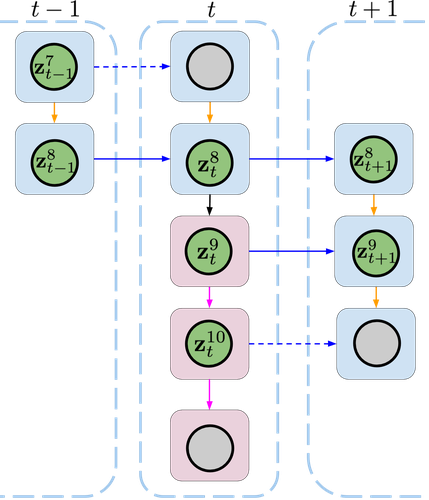
\includegraphics[width=\linewidth]{figures/SQAIR/diagrams/sqair_flow_plus_prop_simple}
    \end{minipage}
    \hfill
    \begin{minipage}[c]{0.49\linewidth}
    \caption{
        \textit{Left}:
            Interaction between \gls{prop} and \gls{disc} in \gls{SQAIR}.
            Firstly, objects are propagated to time $t$, and object $i=7$ is dropped.
            Secondly, \gls{disc} tries to discover new objects.
            Here, it manages to find two objects: $i=9$ and $i=10$.
            The process recurs for all remaining time-steps.
            \textcolor{blue}{Blue arrows} update the temporal hidden state, \textcolor{orange}{orange ones} infer relations between objects, \textcolor{pink}{pink ones} correspond to discovery.
        \textit{Bottom}:
            Information flow in a single discovery block (\textit{left}) and propagation block (\textit{right}). 
            In \gls{disc} we first predict \textit{where} and extract a glimpse. We then predict \textit{what} and \textit{presence}.
            \Gls{prop} starts with extracting a glimpse at a candidate location and updating \textit{where}. Then it follows a procedure similar to \gls{disc}, but takes the respective latent variables from the previous time-step into account. 
            It is approximately two times more computationally expensive than \gls{disc}.
            For details, see \Cref{algo:sqair_prop,algo:sqair_disc} in \Cref{app:algo}.
    }
    \label{fig:sqair_inf_detail}
    \end{minipage}
    \begin{minipage}[c]{0.43\linewidth}
        \centering
        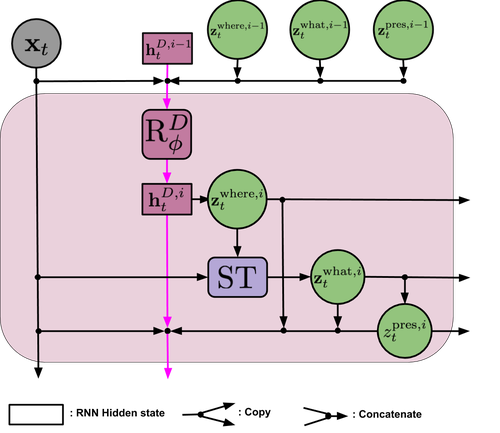
\includegraphics[width=\linewidth]{figures/SQAIR/diagrams/disc}
    \end{minipage}
    \hfill
    \begin{minipage}[c]{0.55\linewidth}
        \centering
        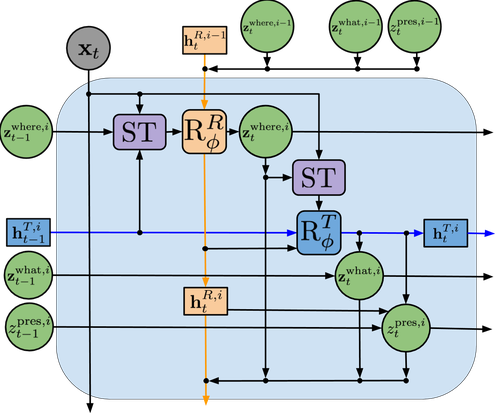
\includegraphics[width=\linewidth]{figures/SQAIR/diagrams/prop}
    \end{minipage}
\end{figure}

\textbf{Inference}
Similarly to \gls{AIR}, inference in \gls{SQAIR} can capture the number of objects and the representation describing the location and appearance of each object that is necessary to explain every image in a sequence.
As with generation, inference is divided into \gls{prop} and \gls{disc}.
During \gls{prop}, the inference network achieves two tasks.
Firstly,
the latent variables from the previous time step are used to infer the current ones, modelling the change in location and appearance of the corresponding objects, thereby attaining temporal consistency. 
This is implemented by the \textit{temporal} \gls{RNN} $\RT$, with hidden states $\textcolor{blue}{\bm{h}_t^T}$ (recurs in $t$). 
Crucially, it does not access the current image directly, but uses the output of the \textit{relation} \gls{RNN} (\textit{cf}. \cite{Santoro2017}).
The relation \gls{RNN} takes relations between objects into account, thereby implementing the \textit{explaining away} phenomenon; 
it is essential for capturing any interactions between objects as well as occlusion (or overlap, if one object is occluded by another). See \Cref{fig:partial_glimpse} for an example.  
These two \gls{RNN}s together decide whether to retain or to forget objects that have been propagated from the previous time step. 
During \gls{disc}, the network infers further latent variables that are needed to describe any new objects that have entered the frame. 
All latent variables remaining after \gls{prop} and \gls{disc} are passed on to the next time step.

See \Cref{fig:sqair_inf_flow,fig:sqair_inf_detail} for the inference network structure .
The full variational posterior is defined as
\vspace{-5pt}
\begin{equation} \label{eq:full_q}
    \q{\Dts, \bzTs}{\bxTs}{\phi} 
        = \prod_{t=1}^T \qd{ \Dt, \bzt^{\mathcal{D}_t} }{ \bxt, \bzt^{\mathcal{P}_t} }{ \phi }
        \prod_{i \in \mathcal{O}_{t-1}} \qp{\bzt^i}{\bz_{t-1}^{i}, \hT{t}{i}, \hR{t}{i}}{\phi}.
\end{equation}
Discovery, described by $\qd_\phi$, is very similar to the full posterior of \gls{AIR}, \textit{cf}. \Cref{eq:air_posterior}.
The only difference is the conditioning on $\bzt^{\mathcal{P}_t}$, which allows for a different number of discovered objects at each time-step and also for objects explained by \gls{prop} not to be explained again.
The second term, or $\qp_\phi$, describes propagation. The detailed structures of $\qd_\phi$ and $\qp_\phi$ are shown in \Cref{fig:sqair_inf_detail}, while all the pertinent algorithms and equations can be found in \Cref{app:algo,apd:sqair_inference}, respectively.

\textbf{Learning}
We train \gls{SQAIR} as an \gls{IWAE} of \cite{Burda2016iwae}. Specifically, we maximise the importance-weighted evidence lower-bound $\loss[\textsc{IWAE}]$, namely

\begin{equation} \label{eq:iwae}
\begin{aligned}
    \loss[\textsc{IWAE}] = \expc[\bxTs \sim \p{\bxTs}{}{\mathrm{data}}]{ 
        \expc[\q]{
            \log \frac{1}{K} \sum_{k=1}^K \frac{ \p{\bxTs, \bzTs}{}{\theta} }{ \q{\bzTs}{\bxTs}{\phi} }   
        }
    }.
\end{aligned}
\end{equation}
To optimise the above, we use \gls{RMSprop}, $K=5$ and batch size of $32$. We use the \textsc{vimco} gradient estimator of \cite{Mnih2016} to backpropagate through the discrete latent variables $z^{\mathrm{pres}}$, and use reparameterisation for the continuous ones \citep{Kingma2014auto}.
We also tried to use \textsc{nvil} of \cite{Mnih2014} as in the original work on \gls{AIR}, but found it very sensitive to hyper-parameters, fragile and generally under-performing.